\documentclass[tikz]{standalone}
\usetikzlibrary{arrows,angles,quotes,calc}
\begin{document}
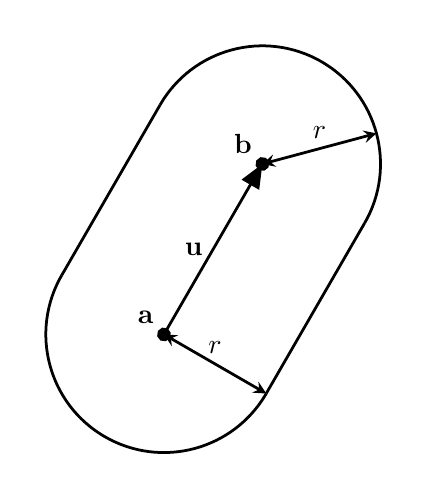
\begin{tikzpicture}[>=triangle 45,line width=1pt,scale=1,font=\fontsize{10pt}{0}]
\coordinate (C) at (0, 0);
\def\R{1.5};
\def\RY{0.75};
\def\H{2.5};

\begin{scope}[xshift=-6cm, rotate=-30]
\draw (0,0) + (\R, 0) 
% arc[start angle=180, end angle=360, x radius=\R, y radius=\RY]
arc[start angle=360, end angle=180, radius=\R];
\draw (0,0) + (\R, \H)
% arc[start angle=180, end angle=360, x radius=\R, y radius=\RY]
arc[start angle=0, end angle=180, radius=\R];

\draw (0,0) +(\R, 0) -- +(\R, \H);
\draw (0,0) +(-\R, 0) -- +(-\R, \H);

\filldraw (0,0) node[anchor=south east] {$\mathbf{a}$} circle (2pt);
\filldraw (0,0) + (0, \H) node[anchor=south east] {$\mathbf{b}$} circle (2pt);

\draw [->] (0,0) -- node[anchor=east] {$\mathbf{u}$} +(0, \H);

\draw [stealth-stealth] (0,0) -- node[anchor=south] {$r$} (\R, 0);
\draw [stealth-stealth] (0,0) ++(0, \H) -- node[anchor=south] {$r$} ++(45:\R);

\end{scope}

\end{tikzpicture}
\end{document}
